\subsection{Activation Functions}

One drawback of the sigmoid function is that its gradients can become very small for large positive or negative inputs, leading to the vanishing gradient problem during backpropagation.
Backpropagation is an optimization algorithm used to minimize the error of neural networks by calculating the gradient of the loss function with respect to each weight through the chain rule and updating the weights accordingly\cite{KELLEY_1960} \cite{Bryson_1962} .

The hyperbolic tangent function is another activation function that provides output values between -1 and 1.
It is defined as:

\begin{align}
  \tanh(z) = \frac{e^z - e^{-z}}{e^z + e^{-z}}
\end{align}

\begin{figure}[H]
  % 
  \centering
  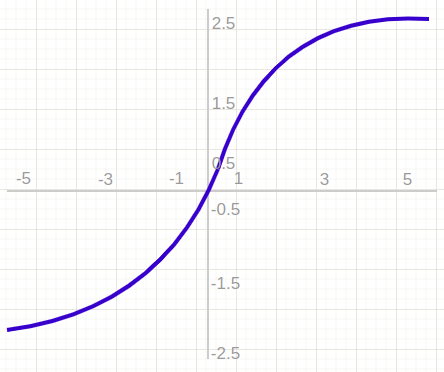
\includegraphics[width=80mm]{figures/tanh.png}
  \caption{tanh Function \cite{Potrimba_2023}}
  \label{tanh}
\end{figure}

In a neural network, a neuron with the tanh activation function computes:

\begin{align}
  \tanh(\sum_i w_i x_i + b) = \frac{e^{(\sum_i w_i x_i + b)} - e^{-(\sum_i w_i x_i + b)}}{e^{(\sum_i w_i x_i + b)} + e^{-(\sum_i w_i x_i + b)}}
\end{align}

The tanh function is zero-centered, which helps in making the learning process faster and more efficient compared to the sigmoid function.
It also suffers from the vanishing gradient problem, though it generally performs better in practice than sigmoid.

The Rectified Linear Unit (ReLU) is a widely used activation function in deep learning models.
It is defined as:

\begin{align}
  \text{ReLU}(z) = \max(0, z)
\end{align}

\begin{figure}[H]
  % 
  \centering
  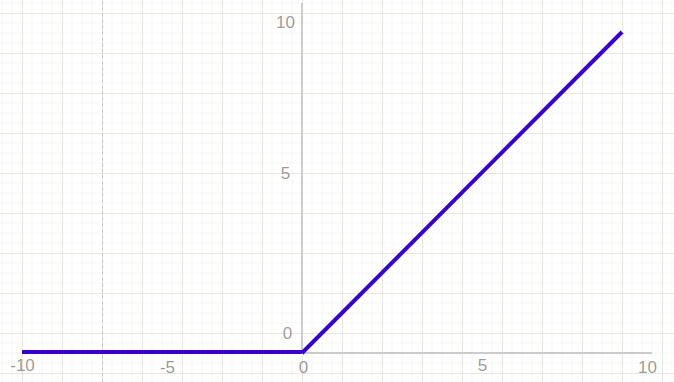
\includegraphics[width=80mm]{figures/relu.png}
  \caption{RELU function \cite{Potrimba_2023}}
  \label{relu}
\end{figure}

For a neuron using ReLU, the output is computed as:

\begin{align}
  \text{ReLU}(\sum_i w_i x_i + b) = \max(0, \sum_i w_i x_i + b)
\end{align}

ReLU introduces non-linearity while being computationally efficient.
It helps mitigate the vanishing gradient problem by allowing gradients to flow more easily through the network\cite{Goodfellow_2016}.
However, it suffers from the "dying ReLU" problem where neurons can sometimes become inactive and only output zero.

To address the dying ReLU problem, the Leaky ReLU function introduces a small, non-zero gradient for negative inputs \cite{Maas_Hannun_Ng_2014}.
It is defined as:

\begin{align}
  \text{Leaky ReLU}(z) = \begin{cases}
    z & \text{if } z > 0 \\
    \alpha z & \text{if } z \leq 0
  \end{cases}
\end{align}

where \( \alpha \) is a small constant (e.g., 0.01).

\begin{figure}[H]
  % 
  \centering
  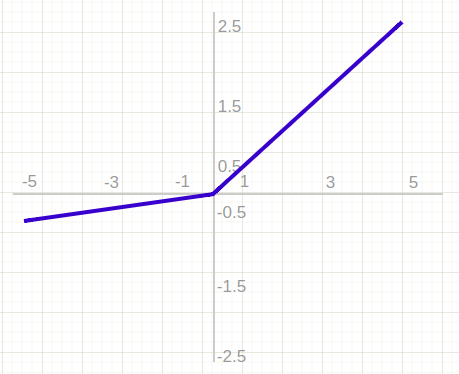
\includegraphics[width=80mm]{figures/lrelu.png}
  \caption{Leaky RELU function \cite{Potrimba_2023}}
  \label{lrelu}
\end{figure}
For a neuron using Leaky ReLU, the output is:

\begin{align}
  \text{Leaky ReLU}(\sum_i w_i x_i + b) = \begin{cases}
    \sum_i w_i x_i + b & \text{if } \sum_i w_i x_i + b > 0 \\
    \alpha (\sum_i w_i x_i + b) & \text{if } \sum_i w_i x_i + b \leq 0
  \end{cases}
\end{align}

The Exponential Linear Unit (ELU) is designed to combine the benefits of ReLU and Leaky ReLU while addressing their limitations.
It is defined as:

\begin{align}
  \text{ELU}(z) = \begin{cases}
    z & \text{if } z > 0 \\
    \alpha (e^z - 1) & \text{if } z \leq 0
  \end{cases}
\end{align}

where \( \alpha \) is a positive constant.

\begin{figure}[H]
  % Different Cite
  % https://www.researchgate.net/figure/The-exponential-linear-unit-ELU-activation-function_fig3_350283420
  \centering
  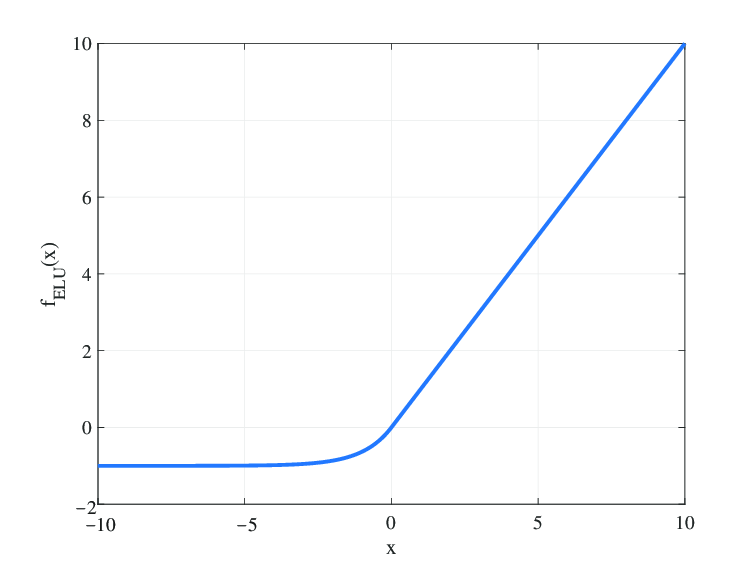
\includegraphics[width=80mm]{figures/elu.png}
  \caption{ELU function \cite{Sheng_2021}}
  \label{elu}
\end{figure}
For a neuron using ELU, the output is:

\begin{align}
  \text{ELU}(\sum_i w_i x_i + b) = \begin{cases}
    \sum_i w_i x_i + b & \text{if } \sum_i w_i x_i + b > 0 \\
    \alpha (e^{(\sum_i w_i x_i + b)} - 1) & \text{if } \sum_i w_i x_i + b \leq 0
  \end{cases}
\end{align}

ELU can help speed up learning and improve robustness to noise by reducing the impact of vanishing gradients.

